\documentclass[handout]{beamer} 
\title{ITCS 531: Number Theory 1 - Prime numbers}
\date{}
\author{Rob Egrot}

\usepackage{amsmath, bbold, bussproofs,graphicx}
\usepackage{mathrsfs}
\usepackage{amsthm}
\usepackage{amssymb}
\usepackage[all]{xy}
\usepackage{multirow}
\usepackage{tikz-cd}


\newtheorem{Def}{Definition}
\newtheorem{Lem}{Lemma}
\newtheorem{Thm}{Theorem}
\newtheorem{Cor}{Corollary}
\newtheorem{Ex}{Example}
\newtheorem{Prop}{Proposition}
\newtheorem{Fact}{Fact}
\newtheorem{Que}{Question}

\newcommand{\bN}{\mathbb{N}}
\newcommand{\bZ}{\mathbb{Z}}
\newcommand{\bQ}{\mathbb{Q}}
\newcommand{\bR}{\mathbb{R}}
\newcommand{\bP}{\mathbb{P}}
\newcommand{\HCF}{\mathbf{HCF}}

\newtheorem{proposition}[theorem]{Proposition}{\bfseries}{\itshape}

\addtobeamertemplate{navigation symbols}{}{%
    \usebeamerfont{footline}%
    \usebeamercolor[fg]{footline}%
    \hspace{1em}%
    \insertframenumber/\inserttotalframenumber
}
\setbeamertemplate{theorems}[numbered]
\begin{document}

\begin{frame}
\titlepage
\end{frame}

\begin{frame}
\frametitle{Prime numbers}
\begin{itemize}
\item Prime numbers the elementary particles of arithmetic.
\vspace{0.3cm}
\item I.e. they cannot be divided into smaller pieces, and they are the building blocks for all other numbers.
\vspace{0.3cm}
\item Mathematicians have been fascinated by prime numbers for thousands of years.
\vspace{0.3cm}
\item There are many simple questions about them that need very advanced techniques from abstract mathematics to solve. 
\end{itemize}
\end{frame}

\begin{frame}
\frametitle{Gaps between primes}
\begin{itemize}
\item For example, do you know if there are an infinite number of primes $p$ such that $p+2$ is also prime? 
\vspace{0.3cm}
\item Nobody does (this is the \emph{twin prime conjecture}). 
\vspace{0.3cm}
\item First proved there is \emph{any} finite number $k$ with an infinite number of pairs of primes whose difference is less than $k$ in 2013. 
\vspace{0.3cm}
\item The first proof by Yitang Zhang has $k$ around 70,000,000, but this has been reduced to 246.
\vspace{0.3cm}
\item More relevant in computer science, prime numbers and their properties give us important techniques for encryption.
\end{itemize}
\end{frame}

\begin{frame}
\frametitle{Digression - fruit}
\[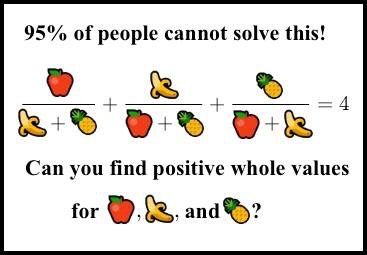
\includegraphics[scale=0.45]{fruit.jpg}\]

\end{frame}

\begin{frame}
\frametitle{Digression - solution}
\begin{itemize}
\item Simplest solution:
\end{itemize}
\vspace{0.3cm}
\tiny
apple = 154476802108746166441951315019919837485664325669565431700026634898253202035277999\\
banana = 36875131794129999827197811565225474825492979968971970996283137471637224634055579\\
pineapple = 4373612677928697257861252602371390152816537558161613618621437993378423467772036\\
\normalsize
\vspace{0.3cm}
\begin{itemize}
\item Brute force search will fail.
\item Need heavy mathematics. 
\item More at: \url{https://www.quora.com/How-do-you-find-the-integer-solutions-to-frac-x-y+z-+-frac-y-z+x-+-frac-z-x+y-4/answer/Alon-Amit}.
\end{itemize}
\end{frame}

\begin{frame}
\frametitle{Notation for sets}
\begin{itemize}
\item $\bN$ is the set \textbf{natural numbers}, so $\bN=\{0,1,2,\ldots\}$.
\vspace{0.3cm}
\item $\bZ$ is the set of \textbf{integers}, so $\bZ=\{\ldots,-2,-1,0,1,2,\ldots\}$.
\vspace{0.3cm}
\item $\bQ$ is the set of \textbf{rational numbers}. $\bQ$ can be thought of as the set of fractions of two integers.
\vspace{0.3cm}
\item $\bR$ is the set of \textbf{real numbers}. $\bR$ can be thought of as the set of all numbers expressible as a (possibly infinite) decimal. 
\vspace{0.3cm}
\item Every real number that is not rational is \textbf{irrational}.
\vspace{0.3cm}
\item If $X$ is a set and $x$ is an element, we use $x\in X$ to say that $x$ is a member of $X$.

\end{itemize}
\end{frame}

\begin{frame}
\frametitle{What is a prime number?}
\begin{itemize}
\item Given two integers $a,b\in \bZ$, we say $a$ divides $b$ if there is $c\in \bZ$ with $b=ac$. 
\vspace{0.3cm}
\item We write $a\mid b$ if $a$ divides $b$. 
\vspace{0.3cm}
\item If $a$ does not divide $b$ we write $a\nmid b$.
\end{itemize}

\begin{definition}[Prime number]
$n\in \bN$ is \emph{prime} if $n>1$ and, whenever $a,b\in \bN$, if $ab=n$ then either $a=1$ and $b= n$ or vice-versa.
\end{definition}

\begin{itemize}
\item We use $\bP$ for the set of prime numbers.
\begin{itemize} 
\item So $\bP=\{2,3,5,7,11,\ldots\}$.  
\end{itemize}
\item Numbers that are not prime are \textbf{composite}.
\end{itemize}

\end{frame}

\begin{frame}
\frametitle{What is to be done}
In this class we will prove two important results about prime numbers which were known to the ancient Greeks.
\vspace{0.5cm}
\begin{theorem}[Fundamental Theorem of Arithmetic]\label{T:fund}
Every natural number greater than 1 can be expressed as a product of primes. Moreover, this product is unique up to reordering.
\end{theorem}
\vspace{0.5cm}
\begin{theorem}\label{T:inf}
The set of prime numbers is infinite.
\end{theorem}
\vspace{0.5cm}
We will need some facts about numbers
\end{frame}

\begin{frame}
\frametitle{Digression - why prove?}
\begin{itemize}
\item Modern mathematicians are obsessed with proof.
\vspace{0.3cm}
\item This goes back to the Ancient Greeks, e.g. as seen in e.g. Euclid.
\vspace{0.3cm}
\item Some Greeks had a religious interest in mathematics (e.g. Pythagoras and his school).
\vspace{0.3cm}
\item Other earlier cultures applied mathematics, e.g. in Egypt, Mesopotamia, China.
\vspace{0.3cm}
\item But these cultures did not emphasize theoretical proof over observation.
\vspace{0.3cm}
\item So why is proof so valued today?
\end{itemize}
\end{frame}

\begin{frame}
\frametitle{Digression - the road to modern mathematics}
\begin{itemize}
\item This is actually a modern phenomena.
\vspace{0.2cm}
\item Although Western mathematics is inspired by Ancient Greece, till the mid 19th century proofs were often not rigorous at all.
\vspace{0.2cm}
\item As math becomes more complicated, more precision is needed for understanding.
\vspace{0.2cm}
\item Also, even easy to understand things that look true turn out to be false.
\vspace{0.2cm}
\item E.g. ``there are no positive integers $a,b,c$ such that $\frac{a}{b+c} + \frac{b}{a+c} + \frac{c}{a+b} = 4$".
\vspace{0.2cm}
\item Experiments with `small' numbers will tell you this is true, but we know it is false.
\end{itemize}
\end{frame}

\begin{frame}
\frametitle{Division of sums}
\begin{lemma}\label{L:plus}
Let $a,b_1,\ldots,b_n\in\bZ$. Then, if $a|b_i$ for all $i\in \{1,\ldots,n\}$, we have $a|(b_1+\ldots +b_n)$.
\end{lemma}
\begin{proof}
\begin{itemize}
\item For each $i\in\{1,\ldots,n\}$ there is $k_i$ with $b_i=k_ia_i$ (by definition of $a|b_i$). 
\item So $b_1+\ldots +b_n = k_1a+\ldots + k_n a = (k_1+\ldots + k_n)a$. 
\item And so $a|(b_1+\ldots+b_n)$ as claimed. 
\end{itemize}
\end{proof}
\begin{itemize}
\item Is the converse true?
\item I.e. if $a|(b_1+\ldots +b_n)$ is it always true that $a|b_i$ for all $i\in\{1,\ldots n\}$?
\item No. e.g. $2|(1+3)$, but $2$ doesn't divide either 1 or 3.
\end{itemize}
\end{frame}

\begin{frame}
\frametitle{Another lemma}
\begin{lemma}\label{L:div1}
Let $a,b,c\in \bZ$. Then if $a|b$ and $a|(b+c)$ then $a|c$.
\end{lemma}
\begin{proof}
\begin{itemize}
\item By definition there are $x,y\in \bZ$ with $xa=b$ and $ya= b+c$. 
\vspace{0.3cm}
\item So combining these we get $ya=xa +c$. 
\vspace{0.3cm}
\item And so $(y-x)a=c$, and so $a|c$ by definition.
\end{itemize}
\end{proof}
\end{frame}

\begin{frame}
\frametitle{Yet another lemma}
\begin{lemma}\label{L:euclid}
Given $a,b\in\bN$ with $a<b$, if $c$ is the highest common factor of $a$ and $b$, then $c$ is also the highest common factor of $b-a$ and $a$.
\end{lemma}
\begin{proof}
\begin{itemize}
\item By definition there are $x,y\in\bN$ with $xc = a$ and $yc= b$. 
\item So $(y-x)c = b - a$, and so $c|(b-a)$. 
\item I.e. $c$ is a common factor of $b-a$ and $a$, and we must show it is the largest such factor. 
\item If $d|(b-a)$ and $d|a$, then by lemma \ref{L:plus} we must have $d|b$. 
\item And so $d\leq c$ as $c$ is the highest common factor of $a$ and $b$. 
\item So $c$ is the highest common factor of $b-a$ and $a$ as required.
\end{itemize}
\end{proof}
\end{frame}

\begin{frame}
\frametitle{The Euclidean algorithm}
\begin{proposition}[Euclid's algorithm]
Given $a,b\in\bN$ with $a< b$ we can find $\HCF(a,b)$ by computing:
\begin{align*}
b &= x_0 a + r_0 \text{ where $r_0< a$} \\
a &= x_1 r_0 + r_1 \text{ where $r_1< r_0$} \\
r_0&=x_2 r_1 + r_2 \text{ where $r_2< r_1$}\\
&.\\
&.\\
&.\\
r_{n-3} &= x_{n-1}r_{n-2} + r_{n-1}\text{ where $r_{n-1}< r_{n-2}$}\\
r_{n-2}&= x_{n} r_{n-1} + r_n \text{ where $r_n< r_{n-1}$} \\
r_{n-1}&= x_{n+1} r_n
\end{align*}
In which case the HCF is $r_n$.
\end{proposition}
\end{frame}

\begin{frame}
\frametitle{The Euclidean algorithm - proof}
\begin{itemize}
\item The algorithm must terminate, because $r_i < r_{i-1}$, so at some point must reach zero. 
\vspace{0.2cm}
\item $r_0$ is found by subtracting $a$ from $b$ multiple times. 
\vspace{0.2cm}
\item So, if $c$ is the HCF of $a$ and $b$, then it is also the HCF of $a$ and $b-a$, and of $a$ and $b-2a$ etc. (lemma \ref{L:euclid}). 
\vspace{0.2cm}
\item So also of $a$ and $r_0$, as $r_0 = b- x_0a$. 
\vspace{0.2cm}
\item By the same logic, the HCF of $a$ and $r_0$ must also be the HCF of $r_0$ and $r_1$. 
\vspace{0.2cm}
\item Continuing this thought process we see that the HCF of $a$ and $b$ must also be the HCF of $r_{n-1}$ and $r_n$.
\vspace{0.2cm}
\item This can only be $r_n$, as $r_n<r_{n-1}$. 
\end{itemize}
\end{frame}

\begin{frame}
\frametitle{The Euclidean algorithm - another proof}
\begin{itemize}
\item $r_n$ divides $r_{n-1}$.
\vspace{0.2cm}
\item So $r_n$ also divides $r_{n-2}$ (lemma \ref{L:plus}).  
\vspace{0.2cm}
\item Similarly $r_n$ divides $r_{n-3}$ etc. 
\vspace{0.2cm}
\item So $r_n|a$ and $r_n|b$.
\vspace{0.2cm}
\item If $d|a$ and $d|b$ then $d|r_0$ (lemma \ref{L:div1}). 
\vspace{0.2cm}
\item Similarly $d|r_1$ etc.
\vspace{0.2cm}
\item So $d|r_n$.
\vspace{0.2cm}
\item I.e. $r_n$ is HCF of $a$ and $b$.
\end{itemize}
\end{frame}

\begin{frame}
\frametitle{The extended Euclidean algorithm}
\begin{corollary}[B\'ezout's identity]\label{C:bez}
If $a,b\in\bN$ and $\HCF(a,b)=d$, then there are $x,y\in \bZ$ such that $d= xa + yb$. 
\end{corollary}
\begin{proof}
\begin{itemize}
\item Use Euclid's algorithm in reverse.
\item Start with $d = r_n = r_{n-2} - x_n r_{n-1}$ in the last step and work backwards. 
\item E.g. the first two steps of this calculation give us:
\begin{align*}
r_n&= r_{n-2}-x_nr_{n-1}\\
&= r_{n-2} - x_n(r_{n-3}-x_{n-1}r_{n-2}).
\end{align*}
\item Define $b = r_{-2}$, and $a = r_{-1}$. 
\item For all $i$ we replace $r_i$ with a term containing $r_{i-1}$ and $r_{i-2}$. 
\item We end up with only $a$ and $b$, and no other $r_i$ values.  
\end{itemize}
\end{proof}
\end{frame}

\begin{frame}
\frametitle{Division by primes}
\begin{lemma}\label{L:div2}
Let $p\in \bP$ and let $a,b\in\bN\setminus\{0\}$. Then, if $p|ab$, either $p|a$ or $p|b$.
\end{lemma}
\begin{proof}
\begin{itemize}
\item Suppose $p|ab$ and $p\nmid a$. 
\item Then $\HCF(p,a)=1$, so by corollary \ref{C:bez} there are $x,y\in\bZ$ with $xp+ya = 1$. 
\item But since $xp+ya = 1$ it follows that $xpb+yab = b$, and since $p|xpb$ and $p|yab$, by lemma \ref{L:plus} we must have $p|b$. 
\item A similar argument proves that if $p\nmid b$ then we must have $p|a$. 
\end{itemize}
\end{proof}

This result generalizes to $p|a_1\ldots a_n\implies p|a_i$ for some $i\in \{1,\ldots,n\}$. You can prove this using induction.  
\end{frame}

\begin{frame}
\frametitle{Almost ready}
\begin{itemize}
\item We are almost ready to prove theorems \ref{T:fund} and \ref{T:inf}.
\vspace{0.5cm}
\item We just need one more idea.
\end{itemize}
\end{frame}

\begin{frame}
\frametitle{The well-ordering principle}
\begin{lemma}[Well-ordering principle]\label{L:well}
If $X\subseteq \bN$ and $X\neq \emptyset$, then $X$ has a smallest element. In other words, every non-empty subset of natural numbers has a smallest member.
\end{lemma}
\begin{proof}
\begin{itemize}
\item Since $X$ has at least one element we can pick $x\in X$. 
\item $X$ has a finite number of elements less than or equal to $x$. 
\item One of these must be smaller than all the others.
\end{itemize}
\end{proof}
\end{frame}

\begin{frame}
\frametitle{Induction}
\begin{itemize}
\item The well-ordering principle is essentially mathematical induction. 
\vspace{0.2cm}
\item I.e. From ``true for 0" and ``true for $n$ implies true for $n+1$" conclude ``true for all natural numbers". 
\vspace{0.2cm}
\item Well-ordering says that if a statement is \emph{not} true for some natural number, then there must be a smallest natural number $k$ where it is not true.
\vspace{0.2cm} 
\item To apply well-ordering usually prove that it's impossible for this smallest $k$ to exist for some statement. 
\vspace{0.2cm}
\item Then can conclude that the set of natural numbers for which the statement of interest is true is empty.
\vspace{0.2cm}
\item I.e. the negation of the statement is true for all natural numbers.
\end{itemize}
\end{frame}

\begin{frame}
\frametitle{Proving theorem \ref{T:fund}}
\begin{itemize}
\item There are two parts to this.
\vspace{0.5cm}
\item Existence: we must show that for all $n > 1$ a prime factorization exists.
\vspace{0.5cm}
\item Uniqueness: we must show that any two prime factorizations of $n$ must be the same up to reordering.
\begin{itemize}
\item E.g. $2\times 7\times 2\times 5$ is a reordering of $2\times 2\times 5\times 7$.
\end{itemize}
\end{itemize}
\end{frame}

\begin{frame}
\frametitle{Proving existence}
\begin{itemize}
\item Suppose $n\in \bN$ and has no prime factorization.
\vspace{0.2cm}
\item Then by the well-ordering principle suppose $n$ is the smallest such number. 
\vspace{0.2cm}
\item If $n$ is prime then $n$ is its own prime factorization (contradiction). 
\vspace{0.2cm}
\item So $n$ is composite. 
\vspace{0.2cm}
\item But then $n=ab$ for some non-trivial factors $a$ and $b$. 
\vspace{0.2cm}
\item By minimality of $n$, both $a$ and $b$ have prime factorizations. 
\vspace{0.2cm}
\item These combine to give a prime factorization of $n$. 
\vspace{0.2cm}
\item I.e. if $a=p_1\ldots p_k$ and $b= q_1\ldots q_m$ then $n=p_1\ldots p_kq_1\ldots q_m$. 
\vspace{0.2cm}
\item Contradiction.
\end{itemize}
\end{frame}

\begin{frame}
\frametitle{Proving uniqueness}
\begin{itemize}
\item Suppose $n$ has 2 distinct factorizations as $p_1\ldots p_k$ and $q_1\ldots q_m$. 
\item By well-ordering we assume that $n$ is minimal with this property. 
\item Here $p_i$ and $q_j$ are primes (which may be repeated) for all $1\leq i\leq k$ and $1\leq j\leq m$. 
\item $p_1$ is not equal to $q_i$ for any $i\in\{1,\ldots,m\}$.
\begin{itemize}
\item Otherwise we could divide both factorizations by $p_1$ to obtain a number smaller than $n$. 
\item But unique factorization would fail for this new number. 
\item This would contradict minimality of $n$. 
\end{itemize} 
\item But $p_1|n$, and so $p_1|q_1\ldots q_m$. 
\item So by lemma \ref{L:div2} we must have $p_1|q_j$ for some $j$. 
\item As $q_j$ is prime this means $p_1= q_j$, which cannot happen. 
\end{itemize}
\end{frame}

\begin{frame}
\frametitle{Proving theorem \ref{T:inf}}
\begin{itemize}
\item Suppose there are only a finite number of primes. 
\item Let the set of primes is $\{p_1,\ldots,p_n\}$. 
\item Then consider the number $k=(\prod_{1=1}^n p_i) +1$. 
\item By the existence part of theorem \ref{T:fund} we know there must be a prime number $p$ dividing $k$. 
\item Since $\{p_1,\ldots,p_n\}$ contains all the primes we must have $p=p_j$ for some $j\in\{1,\ldots,n\}$. 
\item But $p_j|k$ and $p_j|\prod_{i=1}^n p_i$. 
\item So by lemma \ref{L:div1} we must have $p_j|1$. 
\item Contradiction.
\item So the set of primes must be infinite.
\end{itemize}
\end{frame}







\end{document}